\documentclass[conference]{IEEEtran}

% correct bad hyphenation here
\hyphenation{op-tical net-works semi-conduc-tor}

\usepackage{graphicx}

% on table
\usepackage{array}

% on equasion
\usepackage[only,varodot]{stmaryrd}
\usepackage[euler]{textgreek}
\usepackage{MnSymbol}

% table footnote
\usepackage{threeparttable}

\graphicspath{{./img/}}


\begin{document}

\title{Survey Of Several Recent Full Adder Designs}

\author{
	\IEEEauthorblockN{Jun Huang}
	\IEEEauthorblockA{
		Gina Cody School of Engineering and Computer Science\\
		Concordia University\\
		Email: youyinnn@foxmail.com
	}
}
\maketitle

\begin{abstract}
	This paper presents three hybrid full adder designs respectively proposed from 2021, 2020, and 2018.
	Those designs are involved in techniques such as XOR-XNOR gate, CMOS, Gate Diffusion Input(GDI), Transmission Gate(TG), and multi-threshold-voltage(MTV).
	For every design, detail of the FA circuit, the goal of the designers, performance simulation results performed by the designers are presented.
	After comparing three designs in terms of power consumption, propagation delay, and transistor count or area overhead,
	After comparing three designs in terms of power consumption, propagation delay, and transistor count or area overhead,
	% FA-x shows 
\end{abstract}

\begin{IEEEkeywords}
	Full Adder, 1-bit Adder, Hybrid, CMOS, MVT, GDI
\end{IEEEkeywords}

\section{Introduction}

% fa的速度对于VLSI来说越来越重要 冒出了很多技术 在各个方面都得到了提升和优化 

Addition operation plays an important role in very-large-scale integration(VLSI) since it is most common and frequently used in arithmetic operations.
With the development of modern technology, more and more techniques and design have emerged,
to pursue a goal of making the chips less performance delay, less silicon area overhead, and less power consumption.
As is discovered that hybrid logic full design has many merits than the single logic design, circuit designers are more interested in hybrid logic.

Recently in 2021, a 22T XOR-XNOR-based hybrid full adder design \cite{20212210429416} was proposed
which uses an XOR-XNOR module combined with the sum-generation module which uses TG technique
and the carry-generation module which use CCMOS technique.
% As the designers discussed, it is a scalable and full-swing FA
% with some performance improvements compared with several existing state-of-the-art FAs.

Back in 2020, an 18T hybrid full adder design \cite{9339799} came out.
This design is also a three modules cell based on a XOR-XNOR circuit.
With this fundamental circuit, two 4T circuits, which use the GDI technique and TG technique respectively, are driven to generate sum and carry.

Further move backward to 2018, a 14T MVT-GDI-based hybrid full adder design was proposed \cite{18743001}.
This 5 modules FA cell adopts GDI logic and MTV transistor logic and also swing restoring gate.

This paper presents all three FA designs in a fixed order
from module design detail to the purpose of FAs designers, and FAs performance simulation results performed by the designers.

In section \ref{sec:2}, the 22T XOR-XNOR-based hybrid FA is discussed as FA-1.
Then in section \ref{sec:3}, the 18T hybrid FA is discussed as FA-2.
Section \ref{sec:4}, the 14T MVT-GDI-based hybrid FA is discussed as FA-3.
After that, in section \ref{sec:5}, the overall comparison of three FA design is presents.
Section \ref{sec:6} gives the conclusion.

% 列举其他找到的设计 但是并不在报告里讨论 因为设计的论文本身提供的信息在不做模拟的情况下难以放在同一个标准下进行比较 或者论文本身缺失了参数信息

\section{FA-1: XOR-XNOR-based Hybrid FA}
\label{sec:2}

\subsection{Design}

The FA-1 \cite{20212210429416} design contains three modules to realize a 1-bit full adder.
Firstly, an XOR-XNOR circuit will take original inputs \(A\) and \(B\) as its input and produce two signals,
one is from the XNOR gate marked as \(S_{xnor\_out}\) and the other is from the XOR gate marked as \( S_{xor\_out}\).
Then, a TG-based circuit as the second module will take both signal and the input carry \(C_{in}\) to calculate the \(Sum\)
while a third module will then use the \(C_{in}\) along with \(A\), \(B\) and signals \(S_{xnor\_out}\), \( S_{xor\_out}\) to generate the carry \(C_{out}\).

Fig. \ref{fig:fa1-bd} presents the block diagram of the design.

\begin{figure}[!ht]
	\centering
	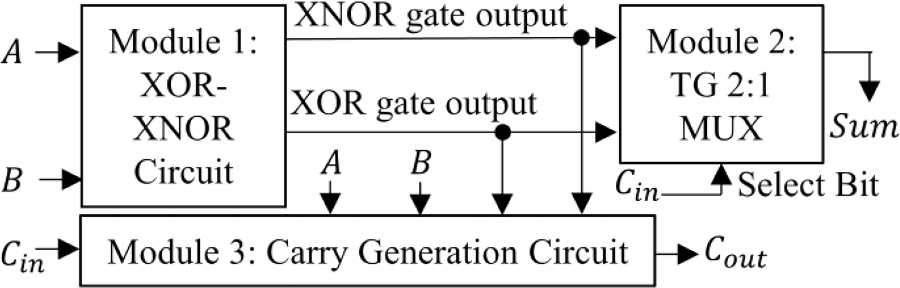
\includegraphics[width=2.7in]{fa1-block diagram.png}
	\caption{Block Diagram of FA-1}
	\label{fig:fa1-bd}
\end{figure}

\subsubsection{Module 1}XOR-XNOR Circuit

The circuit consists of 10 transistors as is shown in Fig. \ref{fig:fa1-xor-xnor}.

\begin{figure}[!ht]
	\centering
	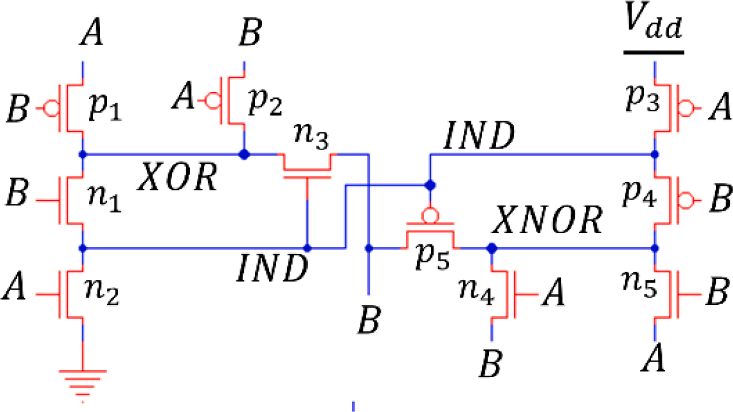
\includegraphics[width=2.2in]{fa1-xor-xnor circuit.png}
	\caption{XOR-XNOR Circuit of FA-1}
	\label{fig:fa1-xor-xnor}
\end{figure}

For all the possible \(A\), \(B\) inputs,
table \ref{tb:xor-xnor} presents all the output patterns also the responsible transistors within the circuit.
As the table presented, it is clear that at least one transistor path can provide full swing output to prevent threshold voltage loss.

\begin{table*}[!htb]
	\renewcommand{\arraystretch}{1.3}
	\caption{Operation Table of the XOR-XNOR circuit of FA-1}
	\centering
	\begin{tabular}{p{1.5cm}p{1.5cm}p{1.5cm}p{4cm}p{4cm}l}
		\hline
		\multicolumn{6}{ c }{\bfseries XOR Circuit}                                                                                                                                                                                     \\
		\multicolumn{3}{ c }{\bfseries Input} & \multicolumn{2}{ c }{\bfseries Output Transistor Path} & \multicolumn{1}{ c }{\bfseries Output}                                                                                         \\
		Pattern no.                           & \(A\)                                                  & \(B\)                                  & Full Swing Transistor Path & Non-Full Swing Transistor Path & Output Signal\(/\)logic \\
		\hline
		1.                                    & 0                                                      & 0                                      & \(n_3\)                    & \(p_1/p_2\)                    & \(B/0\)                 \\
		2.                                    & 0                                                      & 1                                      & \(p_2\)                    & \(n_1/n_3\)                    & \(B/1\)                 \\
		3.                                    & 1                                                      & 0                                      & \(p_1\)                    & None                           & \(A/1\)                 \\
		4.                                    & 1                                                      & 0                                      & \(n_1\) and \(n_2\)        & None                           & \(0\)                   \\
		\hline
		\multicolumn{6}{ c }{\bfseries XNOR Circuit}                                                                                                                                                                                    \\
		\multicolumn{3}{ c }{\bfseries Input} & \multicolumn{2}{ c }{\bfseries Output Transistor Path} & \multicolumn{1}{ c }{\bfseries Output}                                                                                         \\
		Pattern no.                           & \(A\)                                                  & \(B\)                                  & Full Swing Transistor Path & Non-Full Swing Transistor Path & Output Signal\(/\)logic \\
		\hline
		1.                                    & 0                                                      & 0                                      & \(p_3\) and \(p_4\)        & None                           & \(1\)                   \\
		2.                                    & 0                                                      & 1                                      & \(n_5\)                    & None                           & \(A/0\)                 \\
		3.                                    & 1                                                      & 0                                      & \(n_4\)                    & \(p_4/p_5\)                    & \(B/0\)                 \\
		4.                                    & 1                                                      & 0                                      & \(p_5\)                    & \(n_4/n_5\)                    & \(B/1\)                 \\
		\hline
	\end{tabular}
	\label{tb:xor-xnor}
\end{table*}

\subsubsection{Module 2}Sum Generation Circuit

From the Table \ref{tb:fa-tf}, two paths for the Sum generation can be concluded:

when \(C_{in} = 0\):
\[
	Sum = A \oplus B
\]

\begin{table}[!ht]
	\renewcommand{\arraystretch}{1.3}
	\caption{True-False Table of FA}
	\centering
	\begin{tabular}{p{1cm}p{1cm}p{1cm}p{1cm}p{1cm}}
		\hline
		\multicolumn{3}{ c }{\bfseries Inputs} & \multicolumn{2}{ c }{\bfseries Outputs}                                 \\
		\(C_{in}\)                             & \(A\)                                   & \(B\) & \(C_{out}\) & \(Sum\) \\
		\hline
		0                                      & 0                                       & 0     & 0           & 0       \\
		                                       & 0                                       & 1     & 0           & 1       \\
		                                       & 1                                       & 0     & 0           & 1       \\
		                                       & 1                                       & 1     & 1           & 0       \\
		1                                      & 0                                       & 0     & 0           & 1       \\
		                                       & 0                                       & 1     & 1           & 0       \\
		                                       & 1                                       & 0     & 1           & 0       \\
		                                       & 1                                       & 1     & 1           & 1       \\
		\hline
	\end{tabular}
	\label{tb:fa-tf}
\end{table}

when \(C_{in} = 1\):
\[
	Sum = A \varodot B
\]


For input selection, a 2:1 Multiplexer(2:1 MUX) based on Transmission Gate(TG) has been used for figuring the \(Sum\).

As is given in Fig. \ref{fig:fa1-circuit}, two TGs are used for implementing 2:1 MUX logic and with this manner,
the Sum generation circuit can also provide full swing output.

\begin{figure}[!ht]
	\centering
	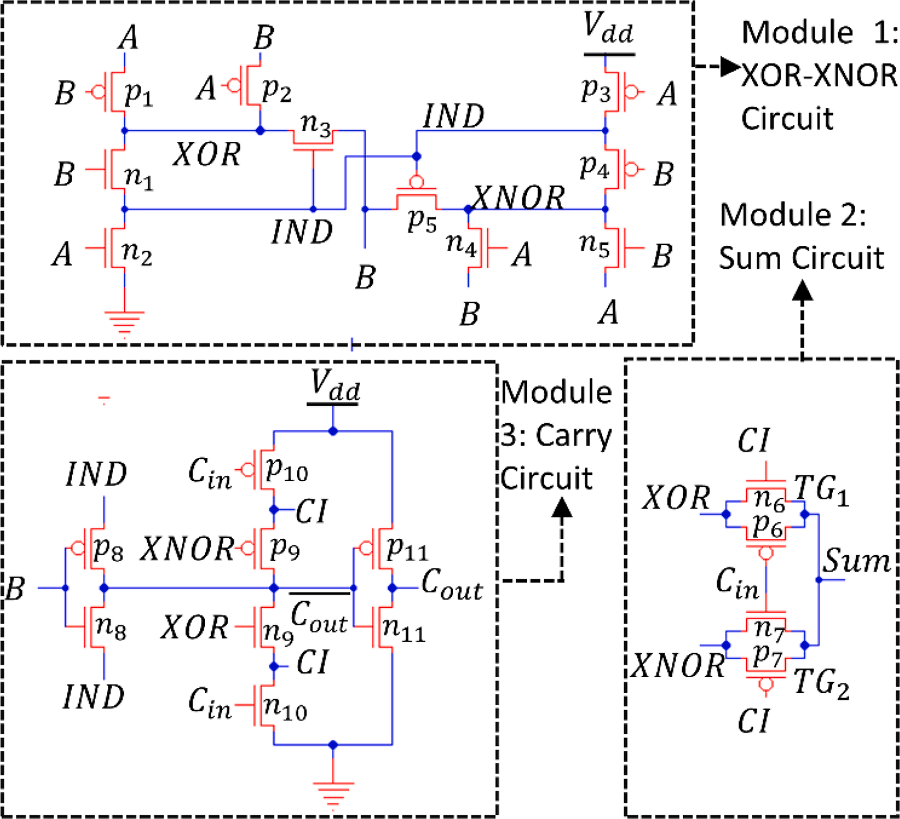
\includegraphics[width=2.7in]{fa1-circuit.png}
	\caption{FA-1 Circuit}
	\label{fig:fa1-circuit}
\end{figure}

\subsubsection{Module 3}Carry Generation Circuit

As per Fig. \ref{fig:fa1-circuit}, the Carry generation circuit uses a CCMOS logic-based inverter at the output.
With this logic, the output voltage level of this circuit is either \(V_{dd}\) or \(G_{nd}\) level.
It is a good design for the extensibility of the circuit
since the design of the carry generation logic is the most important factor of the scalability of the wide word length adders.


\subsection{Discussion}

FA-1 shows impressive improvements compared to many other FAs.
The designers are intended to solve the voltage degradation issue with the hybrid logic-based design,
hence they design the XOR-XNOR-based circuit to produce full swing output for its next stage
and choose TG for implementing the sum generation circuit.

Finally, for the purpose of high-speed calculations and good scalabilities,
they apply the CCMOS technique at the output terminial.
The designed carry generation circuit can be extended to multiple bits adder structures with no additional voltage level restoring buffers.
Furthermore, this logic can reduce the carry chain delay with involving just one pull-up and pull-down transistors.

As for the area overhead, a total of 22 transistors are used to produce this FA, namely, 10 on module one, 4 on module 2, and 8 on module 3.

According to the designers' simulation in terms of average power(AP), propagation delay(PD), area delay product(ADP), power delay product(PDP) on 1-bit FA,
compare with the conventional CMOS FA \cite{weste2015cmos} and other recent FA designs \cite{15484823, 9068497,18743001},
% this design has 19.35\% improvement in Silicon area, 33.59\% improvement in Average Power, 36.15\% improvement in Propagation Delay, 56.22\% improvement in Area Delay Product, and 57.59\% improvement in Power Delay Product.
this design achieves many improvements which can be shown in Table \ref{tb:fa1-comparison}.

\begin{table*}[!ht]
	\begin{threeparttable}[b]
		\renewcommand{\arraystretch}{1.3}
		\caption{Simulations Performed By The Designers of FA-1}
		\centering
		\begin{tabular}{l c p{0.8cm} p{0.8cm} p{0.8cm} p{1.2cm} p{0.8cm} *{5}{p{1cm}}}
			\hline
			\multicolumn{1}{c}{\bfseries FA Cell } & \bfseries TC & \multicolumn{5}{ c }{\bfseries Performance} & \multicolumn{5}{ c }{\bfseries Improvements with Respect to CCMOS FA}                                                                                                                                                             \\
			                                       &              & Area                                        & AP                                                                    & PD             & ADP                      & PDP             &                   &                 &                 &                  &                  \\
			                                       &              & (\textmugreek\(m^2\))                       & (\textmugreek\(W\))                                                   & (ps)           & (\textmugreek\(m^2\).ps) & (\textalpha J)  & Area($\slashdiv$) & AP($\slashdiv$) & PD($\slashdiv$) & ADP($\slashdiv$) & PDP($\slashdiv$) \\
			\hline
			\cite{weste2015cmos} CCMOS             & 28           & 10.13                                       & 1.28                                                                  & 60.3           & 610.84                   & 77.18           & 0.00              & 0.00            & 0.00            & 0.00             & 0.00             \\
			\cite{15484823} Bhattacharyya's        & 16           & 7.58                                        & \bfseries 0.62                                                        & 98.7           & 748.15                   & 61.19           & 25.17             & \bfseries 51.56 & -63.68          & -22.48           & 20.72            \\
			\cite{9068497} Kandpal's               & 20           & 9.18                                        & 0.92                                                                  & 54.06          & 496.27                   & 49.74           & 9.38              & 28.13           & 10.35           & 18.76            & 35.55            \\
			\cite{18743001} Sanapala's             & 14           & \bfseries 7.38                              & 0.75                                                                  & 56.7           & 415.45                   & 42.53           & \bfseries 27.15   & 41.41           & 5.97            & 31.99            & 44.90            \\
			\cite{20212210429416} FA-1             & 22           & 8.17                                        & 0.85                                                                  & \bfseries 38.5 & \bfseries 267.40         & \bfseries 32.73 & 19.35             & 33.59           & \bfseries 36.15 & \bfseries 56.22  & \bfseries 57.59  \\
			\hline
		\end{tabular}
		\begin{tablenotes}
			\item Performed in 1V for 45nm technology
		\end{tablenotes}
		\label{tb:fa1-comparison}
	\end{threeparttable}
\end{table*}


Again, based on the presenters' simulations of the word-length adder architecture \cite{20212210429416},
the FA-1 continues to rank first in these performance comparisons with its scalability advantages,
especially on 16-bit and 32-bit.

\section{FA-2: 18T Hybrid FA}
\label{sec:3}

\subsection{Design}

The FA-2 \cite{9339799} design contains three modules. Same as FA-1 \cite{20212210429416},
the module 1 of the FA-2 is an XOR-XNOR circuit that sending out two signals to drive Module 2 and Module 3 for the calculation of \(Sum\) and \(Carry\).

Module 1 from FA-2 first take \(A\) and \(B\) and produce signal \(H\) (result of $A \oplus B$) and signal $\overline{H}$ (result of $A \varodot B$).
Module 2 then take \(H\) and \(C_{in}\) to calculate the \(Sun\) ($C_{in} \oplus H$).
Module 3 finally figure the \(C_{out}\) out from the input \(A\) and \(C_{in}\) also count in the selection between \(H\) and $\overline{H}$.

The expressions of those outcomes can be:

\[
	Sum = H\overline{C_{in}} + \overline{H}C_{in} = A \oplus B \oplus C_{in}
\]
\[
	C_{out} = HC_{in} + \overline{H}A
\]

\subsubsection{Module 1}XOR-XNOR Circuit

The structure of module 1 is presented in Fig. \ref{fig:fa2-m1}.
To avoid the lack of voltage level, a feedback loop is attached to the XOR output and XNOR output
for reaching the power required to drive the next two modules. So it use a pMOS transistor as Mpf, a nMOS transistor as Mnf.
Any weak logic signal produced by the XOR gate or the XNOR gate (when \(A=B\))
will be handle by the feedback loop and obtains perfect logic signal at the \(H\) or $\overline{H}$ output.
For example, if \(A = B = 0\), weak logic 0 will be produce at the XOR gate as \(H\),
but it still turns ON the Mpf and then logic 1 passes to the Mnf, thus a perfect logic 0 is taken at the \(H\).

\begin{figure}[!hb]
	\centering
	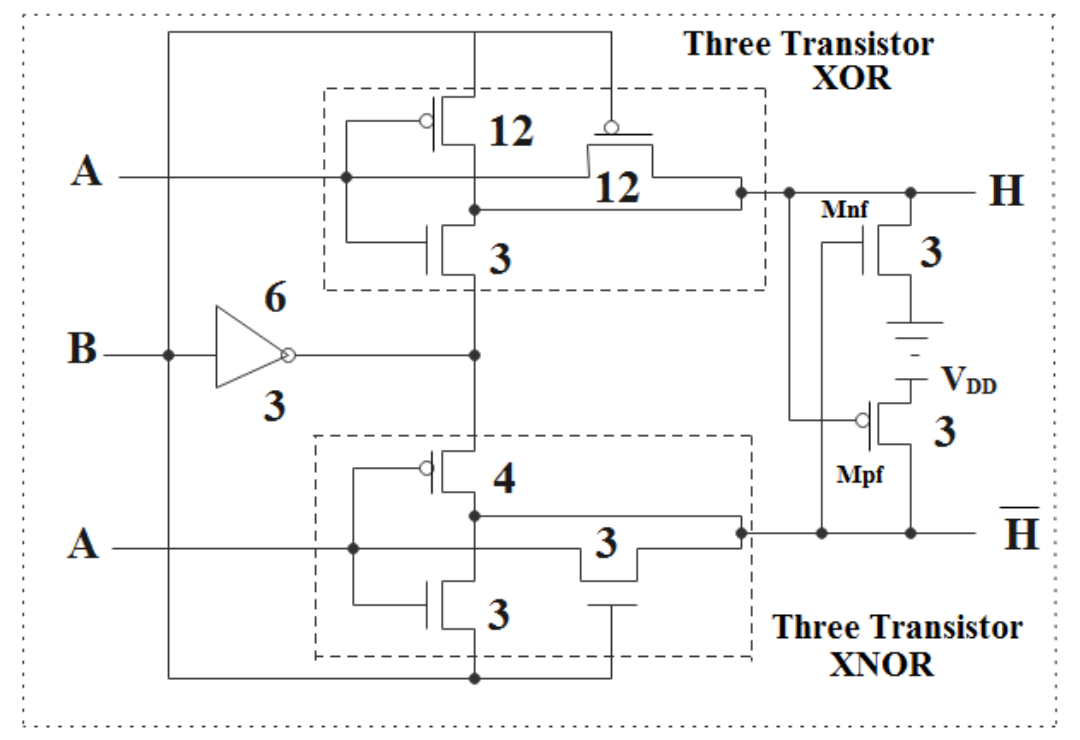
\includegraphics[width=2.7in]{fa2-m1.png}
	\caption{Module 1 of FA-2}
	\label{fig:fa2-m1}
\end{figure}

\subsubsection{Module 2} Sum Generation Circuit

The structure of module 2 is presented in Fig. \ref{fig:fa2-m2}.
Sum generate implementation of FA-2 is an XOR gate with Gate Diffusion Input technique.
So it can generate the full swing output.
When using GDI on the XOR gate, it is required that an inverter provide a perfect signal to the inputs.
But since it retrieves such signal from module 1, the implementation of this module will only need 4 transistors to finish the task.

\begin{figure}[!hb]
	\centering
	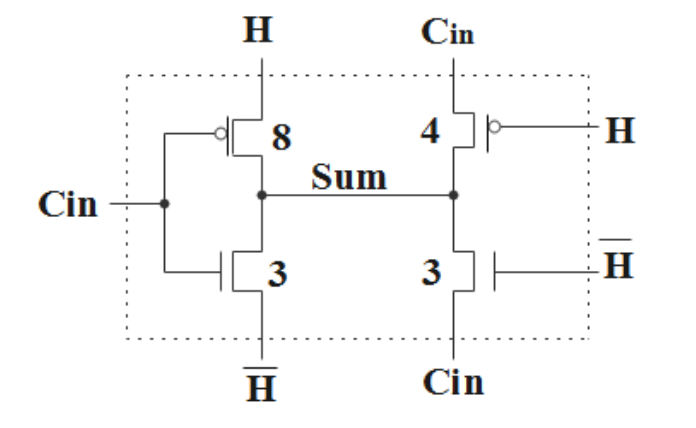
\includegraphics[width=2.4in]{fa2-m2.png}
	\caption{Module 2 of FA-2}
	\label{fig:fa2-m2}
\end{figure}

\subsubsection{Module 2} Carry Generation Circuit

The structure of module 3 is presented in Fig. \ref{fig:fa2-m3}.
The circuit is a 4 pass transistors(PT) 2-to-1 MUX, and it will provide a full swing output by a pMOS and an nMOS conducted in each of the input patterns.
For instance, when \(H = A = 0\), Mp1 and Mn2 turn on, a logic 0 goes through these transistors, \(C_{out}\) obtains perfect 0.

\begin{figure}[!hb]
	\centering
	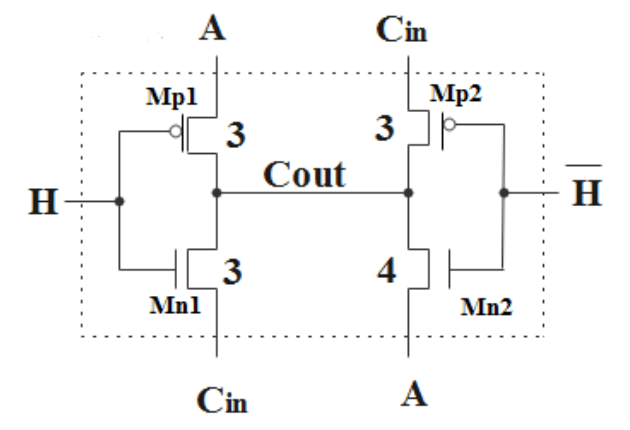
\includegraphics[width=2.4in]{fa2-m3.png}
	\caption{Module 3 of FA-2}
	\label{fig:fa2-m3}
\end{figure}

\subsection{Discussion}

FA-2 design is a lean logic cell for the addition operation.
The designers were well aware of the problems such as bad performance happens at low supply voltages
and the stability of the produced output at different loading conditions.
The design combined feedback loop design, GDI design, and PT technique all together to solve these problems.

With respect of area overhead, 18 transistors are used to bulid this cell. 10 on module 1, 4 on module 2, and 4 on module 3.

As simulations performed by the designers which presented in Table \ref{tb:fa2-comparison},
FA-2 shows its advantages on power consumption, speed, and PDP aspects compared with one old hybrid CMOS FA \cite{9262027} and one hybrid FA \cite{15484823}.

\begin{table}[!ht]
	\begin{threeparttable}[b]
		\centering
		\renewcommand{\arraystretch}{1.3}
		\caption{Simulations Performed By The Designers of FA-2}
		\begin{tabular}{l c *{3}{p{1.2cm}}}
			\hline
			\multicolumn{1}{c}{\bfseries FA Cell } & \bfseries TC & \multicolumn{3}{ c }{\bfseries Performance}                                      \\
			                                       &              & AP(\textmugreek\(W\))                       & PD(ps)          & PDP(fJ)          \\
			\hline
			\cite{9262027} Hybrid CCMOS            & 24           & 6.21                                        & 143             & 0.888            \\
			\cite{15484823} New Hybrid             & 16           & 1.1766                                      & 91.3            & 0.107            \\
			\cite{9339799} FA-2                    & 18           & \bfseries 1.104                             & \bfseries 85.22 & \bfseries 0.0941 \\
			\hline
		\end{tabular}
		\begin{tablenotes}
			\item Performed in 1.2V for 90nm technology
		\end{tablenotes}
		\label{tb:fa2-comparison}
	\end{threeparttable}
\end{table}

\section{FA-3: GDI-based hybrid FA}
\label{sec:4}

\subsection{Design}

The FA-3 \cite{18743001} design, whose structure is illustrated in Fig. \ref{fig:fa3-circuit}, consists of five logic modules.
One XOR/XNOR circuit, two MUX circuits, one Swing Restored Transmission Gate(SRTG) circuit, and one Swing Restored Pass Transistor(SRPT) circuit.

\begin{figure}[!hb]
	\centering
	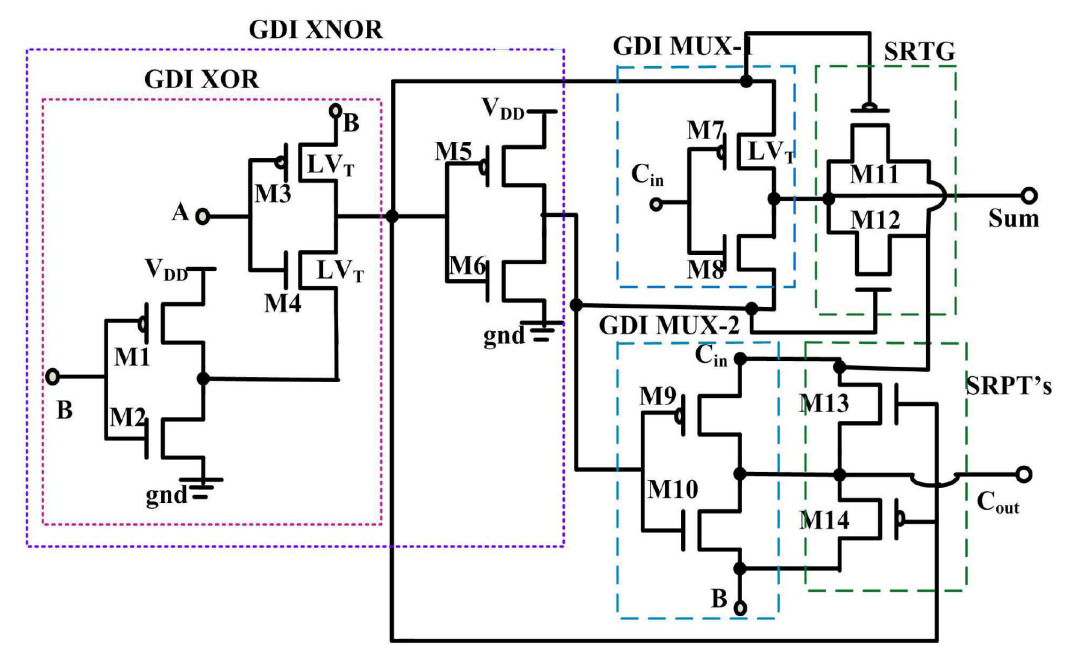
\includegraphics[width=3in]{fa3-circuit.png}
	\caption{FA-3 Circuit}
	\label{fig:fa3-circuit}
\end{figure}

The first module, a XOR/XNOR block, is assembled using GDI design style.
Different from FA-2, module 1 of FA-3 needs a series of inverters to cope with voltage drop issues and, thus, to work with standard \(V_T\)(threshold voltage) devices.

The second module, a GID MUX-1 block, handles the output from both XOR gate and XNOR by a control input \(C_{in}\) then figures the sum out.
So the function can be represented as:

\[
	Sum = \overline{C_{in}}(A \oplus B) + C_{in}(A \varodot B)
\]

The third module, another GID MUX-2 block handles the inputs \(C_{in}\) and \(B\) by control line from the output(\(A \varodot B\)) of XNOR logic.
The function can be represented as:

\[
	C_{out} = (\overline{A \varodot B})C_{in} + (A \varodot B)B
\]

The rest of the two modules are used for full swing logic generation which means a SRTG at the output of the sum and two SRPTs at the carry output.

The functional pattern of the overall circuit is shown in Table \ref{tb:fa3-func-pattern-in} and Table \ref{tb:fa3-func-pattern-out}.

\begin{table}[!ht]
	\renewcommand{\arraystretch}{1.3}
	\caption{The Outputs of The Function table of FA-3}
	\centering
	\begin{tabular}{ c c c }
		\hline
		Input Patterns & Sum                    & \(C_{out}\) \\
		\hline
		1              & 0                      & 0           \\
		2              & 1                      & 0           \\
		3              & 1                      & 0           \\
		4              & 0                      & 1           \\
		5              & \(V_{DD}\)-\(V_T\)(M4) & 0           \\
		6              & 0                      & 1           \\
		7              & 0                      & 1           \\
		8              & 1                      & 1           \\
		\hline
	\end{tabular}
	\label{tb:fa3-func-pattern-out}
\end{table}

\subsection{Discussion}

FA-3 design focuses on providing a full logic swing at ultra-low-voltage(ULV) situation also considering the area overhead and power saving.
To achieve those purposes, the designers choose techniques like multi-threshold voltage(MTV) transistors(in the threshold drop paths),
GDI design style(to reduce the occupied area), and swing restoring gates at the output(for full swing output and faster speed).

Three of the five modules are using GDI technique so that the cell require less transistors to perform the function.

Overall, 14 transistors are used in consists of FA-3, briefly saying, 6 in module 1, rest of each module needs 2 transistors.

The designers perform simulations on FA-3 which can be shown in Table \ref{tb:fa3-comparison}.
Notice that the simulation was conducted at ULV condition, FA-3 has the best performance in terms of delay, energy, and energy delay product(EPD).

\begin{table}[!ht]
	\centering
	\begin{threeparttable}[b]
		\renewcommand{\arraystretch}{1.3}
		\caption{Simulations Performed By The Designers of FA-3}
		\begin{tabular}{l c *{5}{l}}
			\hline
			\multicolumn{1}{c}{\bfseries FA Cell } & \bfseries TC & Area                  & AP             & Delay            & Energy         & EDP             \\
			                                       &              & (\textmugreek\(m^2\)) & (p\(W\))       & (\textmugreek s) & (\textalpha J) & (yJs)           \\
			\hline
			\cite{weste2015cmos} CCMOS             & 28           & 8.536                 & 2.523          & 1.534            & 3.87           & 5.937           \\
			\cite{15484823} 16T Hybrid             & 16           & 7.27                  & 2.506          & 0.978            & 2.451          & 2.397           \\
			\cite{20194307582820} 10-T             & 10           & \bfseries 5.12        & \bfseries 2.34 & 5.95             & 13.923         & 82.84           \\
			\cite{18743001} FA-3                   & 14           & 6.32                  & 3.053          & \bfseries 0.344  & \bfseries 1.05 & \bfseries 0.361 \\
			\hline
		\end{tabular}
		\begin{tablenotes}
			\item Performed in \textbf{ULV of 0.2V} for 45nm technology
		\end{tablenotes}
		\label{tb:fa3-comparison}
	\end{threeparttable}
\end{table}

\begin{table*}[!ht]
	\renewcommand{\arraystretch}{1.3}
	\caption{The Inputs And Signals Of The Function table of FA-3}
	\centering
	\begin{tabular}{ c *{16}{c}}
		\hline
		A B \(C_{in}\) & M1  & M2  & M3  & M4  & \(A \oplus B\)         & M5  & M6  & \(A \varodot B\) & M7  & M8  & M9  & M10 & M11 & M12 & M13 & M14 \\
		\hline
		1: 0 0 0       & ON  & OFF & ON  & OFF & \(V_{T}\)(M3)          & ON  & OFF & 1                & ON  & OFF & OFF & ON  & ON  & ON  & OFF & ON  \\
		2: 0 0 1       & ON  & OFF & ON  & OFF & \(V_{T}\)-\(V_T\)(M3)  & ON  & OFF & 1                & OFF & ON  & OFF & ON  & ON  & ON  & OFF & ON  \\
		3: 0 1 0       & OFF & ON  & ON  & OFF & 1                      & OFF & ON  & 0                & ON  & OFF & ON  & OFF & OFF & OFF & ON  & OFF \\
		4: 0 1 1       & OFF & ON  & ON  & OFF & 1                      & OFF & ON  & 0                & OFF & ON  & ON  & OFF & OFF & OFF & ON  & OFF \\
		5: 1 0 0       & ON  & OFF & OFF & ON  & \(V_{DD}\)-\(V_T\)(M4) & OFF & ON  & 0                & OFF & ON  & ON  & OFF & OFF & OFF & ON  & OFF \\
		6: 1 0 1       & ON  & OFF & OFF & ON  & \(V_{DD}\)-\(V_T\)(M4) & OFF & ON  & 0                & OFF & ON  & ON  & OFF & OFF & OFF & ON  & OFF \\
		7: 1 1 0       & OFF & ON  & OFF & ON  & 0                      & ON  & OFF & 1                & ON  & ON  & OFF & ON  & ON  & ON  & OFF & ON  \\
		8: 1 1 1       & OFF & ON  & OFF & ON  & 0                      & ON  & OFF & 1                & OFF & ON  & OFF & ON  & ON  & ON  & OFF & ON  \\
		\hline
	\end{tabular}
	\label{tb:fa3-func-pattern-in}
\end{table*}

\section{Comparison}
\label{sec:5}

An XOR-XNOR-based hybrid full adder design has been proposed\cite{20212210429416}
which uses an XOR-XNOR module combined with the carry-generation module and the sum-generation module.
As the designers discussed, it is a scalable and full-swing FA
with some performance improvements compared with several existing state-of-the-art FAs.An XOR-XNOR-based hybrid full adder design has been proposed\cite{20212210429416}
which uses an XOR-XNOR module combined with the carry-generation module and the sum-generation module.
As the designers discussed, it is a scalable and full-swing FA
with some performance improvements compared with several existing state-of-the-art FAs.

An XOR-XNOR-based hybrid full adder design has been proposed\cite{20212210429416}
which uses an XOR-XNOR module combined with the carry-generation module and the sum-generation module.
As the designers discussed, it is a scalable and full-swing FA
with some performance improvements compared with several existing state-of-the-art FAs.An XOR-XNOR-based hybrid full adder design has been proposed\cite{20212210429416}
which uses an XOR-XNOR module combined with the carry-generation module and the sum-generation module.
As the designers discussed, it is a scalable and full-swing FA
with some performance improvements compared with several existing state-of-the-art FAs.

An XOR-XNOR-based hybrid full adder design has been proposed\cite{20212210429416}
which uses an XOR-XNOR module combined with the carry-generation module and the sum-generation module.
As the designers discussed, it is a scalable and full-swing FA
with some performance improvements compared with several existing state-of-the-art FAs.An XOR-XNOR-based hybrid full adder design has been proposed\cite{20212210429416}
which uses an XOR-XNOR module combined with the carry-generation module and the sum-generation module.
As the designers discussed, it is a scalable and full-swing FA
with some performance improvements compared with several existing state-of-the-art FAs.

\section{Conclusion}
\label{sec:6}

An XOR-XNOR-based hybrid full adder design has been proposed\cite{20212210429416}
which uses an XOR-XNOR module combined with the carry-generation module and the sum-generation module.
As the designers discussed, it is a scalable and full-swing FA
with some performance improvements compared with several existing state-of-the-art FAs.An XOR-XNOR-based hybrid full adder design has been proposed\cite{20212210429416}
which uses an XOR-XNOR module combined with the carry-generation module and the sum-generation module.
As the designers discussed, it is a scalable and full-swing FA
with some performance improvements compared with several existing state-of-the-art FAs.

\bibliographystyle{ieeetr}
\bibliography{bibliographies}
\end{document}
